{% -*- mode: LaTeX; TeX-PDF-mode: t; TeX-master: "manual"; -*-
}

\chapter{The \ei Output Language}
\label{ch:eiol}

In this chapter we describe a text-based output language that allows
tools to view their output in a graphical way, e.g., highlighting
lines, adding markers, defining on-click actions, etc. The main
advantage of this language is that it does not require any knowledge
on GUI or WEB programming.
%
Some clients, e.g., the web-client described in
Section~\ref{sec:clients:web}, are supposed to support this
language. This is done by developing a corresponding interpret that
renders the effect of the corresponding commands in the respective
environment (e.g., a web browser).

The rest of this chapter is organized as follows: 
%
in Section~\ref{sec:eiol:overview} we first give a general overview of
the design of this language; 
%
in Section~\ref{sec:eiol:spec} we describe the syntax and semantics of
this language; 
%
in Section~\ref{sec:eiol:other} we include some details that we left
out of Section~\ref{sec:eiol:spec} for readability (we refer the
reader to these parts in Section~\ref{sec:eiol:spec}); and 
%
in Section~\ref{sec:eiol:examples} we give some examples to the
different parts of the language.



\section{General Overview}
\label{sec:eiol:overview}

The idea behind the \ei output language is that a tool should just
print, on the standard output, how it wants to view the output using
some high-level description, and leave the details to an interpreter
that converts this description to graphical output.
%
This way we move the complexity of constructing a GUI from the tool to
the interpreter, and thus free developers of tools from mastering any
WEB or GUI related libraries.
%
To simplify the processing of such output, we should use some
structured format. In our case we opt for XML, but we could use any
other structured formatting. e.g., JSON.


The \ei output language assumes that the environment in which it is
interpreted includes:
%
\begin{enumerate}[\upshape(\itshape i\upshape)]

\item A ``\texttt{Code Editor}'' where programs can be edited,
  typically a tab for each file;
%
\item A ``\texttt{File Manager}'' that includes a tree-view of all
  user files and predefined examples;
%
\item A \texttt{Console} where output can be printed in different
  formats (it might include also several consoles, e.g., several
  tabs).
\end{enumerate}
%
An output in the \ei output language is an XML structure of the
following form:

\medskip
\noindent
\begin{lstlisting}
<eiout> 
 <eicommands>
    $\xmlstructref{eiout}{eicommand}$*
 </eicommands>
 <eiactions>
    $\xmlstructref{eiout}{eiaction}$*
 </eiactions>
</eiout>
\end{lstlisting}

\medskip
\noindent
where
\begin{enumerate}[\upshape(\itshape i\upshape)]
\item \lst{eiout} is the outermost tag that encapsulates all commands
  and actions;
\item \xmlstructref{eiout}{eicommand}* is a list of commands to be
  executed; and
\item \xmlstructref{eiout}{eiaction}* is a list of actions to be
  declared. Actions correspond to interactions with the user.
\end{enumerate}
%
Typical examples of \xmlstructref{eiout}{eicommand} are: \emph{print a
  text on the console}, \emph{highlight lines 5-10}, \emph{add marker
  at line 5}, etc.
%
Typical examples of \xmlstructref{eiout}{eiaction} are: \emph{when the
  user clicks on line 13, highlight lines 20-25}, \emph{when the user
  clicks on some text, open a dialog box with some message}, etc.

In the next section we give a detailed specification of this
language. Note that currently the language includes some commands and
actions of interest, that we needed for our tools in the \envisage
project, however, it is design in a way that is easily extensible to
include more commands an actions (interpreters on the client side
should be modified to support such extensions).

\section{Syntax and Semantics}
\label{sec:eiol:spec}


An output in the \ei output language is an XML structure that adhere
to the syntax of \xmlstructref{eiout}{eiout} that is described
below. You can follow the links in its definition in order to get the
definitions of its different parts. 
%
The semantics of each is fully specified, and when needed we refer the
reader to clarifying examples.

\bigskip
\noindent
\textbf{IMPORTANT:} note that the output must be a valid XML
structure, thus, in what follows, whenever we need to include
\emph{plain text} in that output, such text should be enclosed in a
\lst{<![CDATA[ $\mbox{the-text-goes-here}$ ]]>} environment (see
Example~\ref{sec:eiol:examples:4}).


%% EIOUT
%%
\bigskip
\xmlstruct
{eiout}
{eiout} 
{%
%
  This is the main environment of the output, it includes several
  lists of command environments \xmlstructref{eiout}{eicommands}, and
  several lists of action environments \xmlstructref{eiout}{eiactions}.
%
  Commands are executed first, in the given order, and then actions are
  executed in the given order as well.
%
  The \xmlstructattr{version} attribute indicates the version of the
  output language that is used, which is $1.0$ by default.
%
}


%% EICOMMANDS
%% 
\bigskip
\xmlstruct
{eiout}
{eicommands}
{%
%
A list of commands to be performed.
%
The attribute \xmlstructattr{dest} is the destination file on which
the command is applied (if needed), it should be the full path to that
file as provided by the \ei server.
%
E.g., when highlighting a line we might want to highlight a line in
one file or another. 
%
If \xmlstructattr{dest} is not specified, then the commands will be
applied to the file that is currently active, e.g., if the client
includes a code editor with several tabs, one for each file, the
command will be applied to the active tab. If none is active then the
behavior is not specified.
% 
The attribute \xmlstructattr{outclass} specifies the \emph{output
  class} of the commands in this environment, that is, the nature of
the corresponding output generated by the commands, e.g., error,
information, warning, etc. The effect of this attribute is not fully
specified and it depends on the client and the actual implementation
of the interpreter.
%
All commands inside this environment inherit the values of
\xmlstructattr{outclass} and \xmlstructattr{dest}, and each can
override them.
%
}


%% EIACTIONS
%% 
\bigskip
\xmlstruct
{eiout}
{eiactions}
{%
%
  A a list of actions to be declared. An action typically executes a
  list of \xmlstructref{eiout}{eicommands} when the user interacts with the
  interface in some predetermined way, e.g., \emph{when the user
    clicks on line 30, highlight lines number 12 and 16}. We say the
  an action is \emph{performed} as a response to the user interaction.
%
  If the user interacts again with the interface, according to what is
  specified in the action, then the action is \emph{unperformed} if
  possible (when the corresponding commands support the \emph{undo}
  operation), e.g., in the above example if the user clicks again on
  Line 30 again, the highlights of lines 12 and 16 are turned off.

  Before \emph{performing} an action, the last \emph{performed} action
  is \emph{unperformed} first. This behavior can be disabled by
  setting the \xmlstructattr{autoclean} attribute to
  \xmlstructvalue{``false''}. All actions inside this environment
  inherit the value of \xmlstructattr{autoclean}, and each can
  override it.
% 
  The attribute \xmlstructattr{dest} and \xmlstructattr{outclass} are
  as in the case of commands (see the description of
  \xmlstructref{eiout}{eicommands}).
%
}


%% EICOMMAND
%% 
\bigskip
\xmlstruct
{eiout}
{eicommand}
{
A command in the \ei output language, briefly:
\begin{itemize}
\item \xmlstructref{eiout}{printonconsolecommand} can be used to print on the console.
%
\item \xmlstructref{eiout}{highlightlinescommand} can be used to highlight
  lines in the code editor.
%
\item \xmlstructref{eiout}{dialogboxcommand} can be used to open a dialog
  window with a corresponding message.
%
\item \xmlstructref{eiout}{writefilecommand} can be used to add a file (and a
  corresponding content) to the file-manager.
%
\item \xmlstructref{eiout}{setcsscommand} can be used to change the
  CSS properties of some elements that were previously generated
  (e.g., content in HTML)
%
\item \xmlstructref{eiout}{addmarkercommand} can be used to add a marker next
  to a line in the code editor.
%
\item \xmlstructref{eiout}{addinlinemarkercommand} can be used to add a line
  widget (an inlined marker) in the code editor.
%
%% \item \xmlstructref{eiout}{streamcommand} can be used to notify that
%%   there is an stream application running.
%
\item \xmlstructref{eiout}{downloadcommand} can be used to download a
  file that was previously generated by a tool.
%
\item \xmlstructref{eiout}{changecontentcommand} can be used to modify
  a content that has been previously generated.
%
\end{itemize}
}


%% EIACTION
%% 
\bigskip
\xmlstruct
{eiout}
{eiaction}
{%
An action in the \ei output language, briefly:
\begin{itemize}
%
\item \xmlstructref{eiout}{oncodelineclickaction} can be used to perform an action
  when the user clicks on a line in the code editor.
%
\item \xmlstructref{eiout}{onclickaction} can be used to perform an
  action when the user clicks on a previously generated text (a DOM
  element in general).
%
%% \item \xmlstructref{eiout}{timelineaction} TO-DO.
%
\end{itemize}
}


%% PRINTONCONSOLECOMAND
%%
\bigskip
\xmlstruct
{eiout}
{printonconsolecommand}
{%
%
  Prints the content described by the \xmlstructref{eiout}{content}
  environments on the console that has an identifier
  \xmlstructattr{consoleid}.
%
  If \xmlstructattr{consoleid} is not specified, the output goes to
  the default console.
%
  If \xmlstructattr{consoleid} is specified but there is no console
  with such an identifier, the console is created and
  \xmlstructattr{consoletitle} (if specified) is used as its title.
%
  The attribute \xmlstructattr{outclass} is as described in
  \xmlstructref{eiout}{eicommands}.
%
  \\\\See Example~\ref{sec:eiol:examples:1}.
} 

%% HIGHLIGHTLINESCOMMAND
%%
\bigskip
\xmlstruct
{eiout}
{highlightlinescommand}
{%
%
  Highlights the lines specified by \xmlstructref{eiout}{lines} in the
  file \xmlstructattr{dest}. The attribute \xmlstructattr{outclass} is
  as described in \xmlstructref{eiout}{eicommands}.
%
  \\\\See Example~\ref{sec:eiol:examples:2}.
}

%% DIALOGBOXCOMMAND
%%
\bigskip
\xmlstruct
{eiout}
{dialogboxcommand}
{%
  Opens a dialog box with the content specified by the
  \xmlstructref{eiout}{content} environments. The value of
  \xmlstructattr{boxtitle}, if specified, is used as a title for the
  dialog box. The attributes \xmlstructattr{boxwidth} and
  \xmlstructattr{boxheight} can be used to set the size of the window.
  The attribute \xmlstructattr{outclass} is as in
  \xmlstructref{eiout}{eicommands}.
%
  \\\\See Example~\ref{sec:eiol:examples:3}.
}


%% WRITEFILECOMMAND
%%
\bigskip 
\xmlstruct 
{eiout}
{writefilecommand} 
{%
%
  Creates a new file it in the file-manager, using the path specified
  by \xmlstructattr{filename}. The file's content is set to the value
  of \xmlstructref{eiout}{text}. If the file exists, and
  \xmlstructattr{overwrite} is \xmlstructvalue{true}, the content is
  replaced otherwise a new file is created with a new name. The
  default value of \xmlstructattr{overwrite} is
  \xmlstructvalue{false}.
% 
%  This command does not support \emph{undo}.
%
  \\\\See Example~\ref{sec:eiol:examples:4}.
}


%% SETCSSCOMMAND
%%
\bigskip
\xmlstruct
{eiout}
{setcsscommand}
{%
%
  Changes the CSS properties, as specified by
  \xmlstructref{eiout}{cssproperties}, of all elements that match the
  selectors in \xmlstructref{eiout}{elements}.
%
  There must be exactly one \xmlstructref{eiout}{elements} environment and
  one \xmlstructref{eiout}{cssproperties} environment. 
%
  The elements are selected from those that were previously generated
  by other commands.
%
  \\\\See Example~\ref{sec:eiol:examples:5}.
}

%% CHANGECONTENTCOMMAND
%%
\bigskip
\xmlstruct
{eiout}
{changecontentcommand}
{%
% 
  Modifies the content of all elements that match the selectors in
  \xmlstructref{eiout}{elements}, using
  \xmlstructref{eiout}{content}. These elements are typically selected
  from those generated by previously executed commands.
%
  The attribute \xmlstructattr{action} indicates how to incorporate
  \xmlstructref{eiout}{content} in the current one, i.e.,
  \xmlstructvalue{replace}, \xmlstructvalue{append} or
  \xmlstructvalue{prepend}.
%
  \\\\See Example~\ref{sec:eiol:examples:6}.
}

%% ADDMARKERCOMMAND
%%
\bigskip
\xmlstruct
{eiout}
{addmarkercommand}
{%
%
  Adds a marker next to each line that is specified in
  \xmlstructref{eiout}{lines}. The column information from each
  \xmlstructref{eiout}{line} in \xmlstructref{eiout}{lines} is
  ignored.  All markers are associated with the content given by the
  \xmlstructref{eiout}{content} environments, as a tooltip for
  example. If the client allows expanding the tooltip to a dialog
  window, the attributes \xmlstructattr{boxtitle},
  \xmlstructattr{boxwidth} and \xmlstructattr{boxheight} can be used
  to set the properties of the corresponding window (see
  \xmlstructref{eiout}{dialogboxcommand}).
%
  If a line is already associated with a marker, then all
  \xmlstructref{eiout}{content} environments should be appended to the
  current content.
%
  The attributes \xmlstructattr{dest} and \xmlstructattr{outclass} are
  as described in \xmlstructref{eiout}{eicommands}.
%
  \\\\See Example~\ref{sec:eiol:examples:7}.
}

\bigskip
\xmlstruct
{eiout}
{addinlinemarkercommand}
{%
%
  Adds an inline marker (a line widget) for each line that is
  specified by \xmlstructref{eiout}{lines}. All line widgets will
  include the content specified by the \xmlstructref{eiout}{content}
  environments. The column information from each
  \xmlstructref{eiout}{line} in \xmlstructref{eiout}{lines} is
  ignored.
%
  If a line is already associated with a marker, then all
  \xmlstructref{eiout}{content} environments should be appended to the
  current content.
%
  The attributes \xmlstructattr{dest} and \xmlstructattr{outclass} are
  as described in \xmlstructref{eiout}{eicommands}.
%
  \\\\See Example~\ref{sec:eiol:examples:8}.
}

%% STREAM COMMAND
%% \bigskip
%% \xmlstruct
%% {eiout}
%% {streamcommand}
%% {%
%% %
%%   Notify that there is an application running and you can get their
%%   results each \xmlstructattr{time} seconds asking to the ei server
%%   with the \xmlstructattr{execid} given.
%%   %
%%   Also the \xmlstructref{eiout}{content} of the command will be
%%   printed on the console \xmlstructattr{consoleid} that print all the
%%   stream data. 
%% %
%% }

%% DOWNLOADCOMMAND
%%
\bigskip
\xmlstruct
{eiout}
{downloadcommand}
{%
%
  When a tool that runs on an \ei server X generates this command, the
  effect should be downloading the file specified in
  \xmlstructattr{filename}, from the \ei server X, using the execution
  identifier \xmlstructattr{execid}. See
  sections~\ref{sec:server:config:workflow} and
  \ref{sec:server:access:download} for more information on downloading
  files from an \ei server.
%
  \\\\See Example~\ref{sec:eiol:examples:9}.
}

%% ONCODELINECLICKACTION
%%
\bigskip
\xmlstruct
{eiout}
{oncodelineclickaction}
{%
%
  Adds (special) markers at the code lines specified by
  \xmlstructref{eiout}{lines}, such that when any is clicked the
  commands in \xmlstructref{eiout}{eicommands} are performed, and if
  clicked again they are unperformed (see detailed description in
  \xmlstructref{eiout}{eiactions}).
  % 
  The content given by the \xmlstructref{eiout}{content} environments is
  associated with the markers (as a tooltip for example).
%
  If a line is already associated with such an action, then
  \xmlstructref{eiout}{content} should be appended to the current
  content and \xmlstructref{eiout}{eicommands} should be accumulated
  to the current ones.
%
  The attributes \xmlstructattr{dest}, \xmlstructattr{outclass} and
  \xmlstructattr{autoclean} are as described in
  \xmlstructref{eiout}{eiactions}. Moreover, the
  \xmlstructref{eiout}{eicommands} environment inherits the
  \xmlstructattr{dest} and \xmlstructattr{outclass} attributes of this
  environment.
%
  \\\\See Example~\ref{sec:eiol:examples:2}.
}%

\bigskip
\xmlstruct
{eiout}
{onclickaction}
{%
%
  A click on any element that matches any selector from
  \xmlstructref{eiout}{elements} will execute the commands declared in
  \xmlstructref{eiout}{eicommands}, and if clicked again they are
  unperformed (see detailed description in
  \xmlstructref{eiout}{eiactions}).
%
  If the element is already associated with an action, then
  \xmlstructref{eiout}{eicommands} should be accumulated to the
  current ones.
%
%
  The attributes \xmlstructattr{dest}, \xmlstructattr{outclass} and
  \xmlstructattr{autoclean} are as described in
  \xmlstructref{eiout}{eiactions}. Moreover, the above
  \xmlstructref{eiout}{eicommands} environment inherits the
  \xmlstructattr{dest} and \xmlstructattr{outclass} attributes of this
  environment.
%
  \\\\See Example~\ref{sec:eiol:examples:5}.
}%

%% \bigskip
%% \xmlstruct
%% {eiout}
%% {timelineaction}
%% {%
%% %
%%   TO-DO
%% %
%% }

%% %%
%% \bigskip
%% \xmlstruct
%% {eiout}
%% {step}
%% {%
%% step of timeline
%% }


%% 
\bigskip
\xmlstruct
{eiout}
{lines}
{%
%
A group of lines, typically used to specify the lines affected by 
an \xmlstructref{eiout}{eicommand} or an \xmlstructref{eiout}{eiaction}.
%
}


%% 
\bigskip
\xmlstruct
{eiout}
{line}
{%
%
  A region (of lines) typically used to specify the region on which
  the effect of an \xmlstructref{eiout}{eicommand} or an
  \xmlstructref{eiout}{eiaction} is applied:
%
\begin{itemize}
\item \xmlstructattr{from} is the start line.
\item \xmlstructattr{to} is the end line.
\item \xmlstructattr{fromch} is the character (i.e., column number)
  where the first line starts.
\item \xmlstructattr{toch} is the character (i.e., column number)
  where the last line ends.
\end{itemize}
%
The default value of \xmlstructattr{to} is as the value of
\xmlstructattr{from}. The default value of \xmlstructattr{fromch} is
0, and of \xmlstructattr{toch} is the end of the line.
%
}


\bigskip
\xmlstruct
{eiout}
{elements}
{%
  Set of selectors (of DOM elements)
} 

\bigskip
\xmlstruct
{eiout}
{selector}
{%
%
  The attribute \xmlstructattr{value} must be a valid selector as in
  jQuery (see \url{https://jquery.com}). It is used to match some DOM
  elements.
%
}


\bigskip
\xmlstruct
{eiout}
{cssproperties}
{%
%
A set of CSS properties.
%
}


\bigskip
\xmlstruct
{eiout}
{cssproperty}
{%
%
  A CSS property. The attributes \xmlstructattr{name} and
  \xmlstructattr{value} should correspond to valid CSS properties.
%
}


%% CONTENT
\bigskip
\xmlstruct
{eiout}
{content}
{%
%
  A text \xmlstructref{eiout}{text} given in a specific
  \xmlstructattr{format}, that is supposed to be viewed to the
  user. If the attribute \xmlstructattr{format} is not provided, then
  it is assumed to be in \xmlstructvalue{"text"} format (plain text).
%
  This content should be viewed to the user in the specified
  format. The supported formats are:
%
\begin{itemize}
\item \xmlstructvalue{"text"}, for plain text;
\item \xmlstructvalue{"html"}, for HTML;
\item \xmlstructvalue{"svg"}, for Scalable Vector Graphics~\cite{svg}; and
\item \xmlstructvalue{"graph"}, for drawing 2D graphs -- see
  Section~\ref{sec:eiol:other:graph} for the exact
  format.
\end{itemize}
%
The rest of attributes can be used to associate the content with an
output stream as follows (first see
sections~\ref{sec:server:config:workflow} and
\ref{sec:server:access:stream} to understand the notions behind
streaming before you continue):
%
\begin{itemize}
\item \xmlstructattr{execid} is the execution identifier;
\item \xmlstructattr{ext} is the extension of output chunk files to be
  retrieved;
\item \xmlstructattr{action} indicates how to incorporate new output
  chunks to the current content (i.e., \xmlstructvalue{replace},
  \xmlstructvalue{append} or \xmlstructvalue{prepend}); and
\item \xmlstructattr{refreshrate} is a time interval (in seconds) to
  be used for refreshing the output. If the value is not specified
  then refreshing the output should be on demand.
\end{itemize}
%
The client should stop refreshing when the background processes of the
corresponding stream have terminated, or when the user asks to stop
them explicitly.
%
}%

\bigskip
\noindent
\xmlstructdef{eiout}{consoleid}

( [a-z,A-Z,0-9,-,\_]+ | \lst{$\mbox{new}$} | \lst{$\mbox{default}$} )

\medskip
\noindent
The value \lst{$\mbox{new}$} means a new console, we cannot refer to
this console later. The value \lst{$\mbox{default}$} means the default
console of the client.


\bigskip
\noindent
\xmlstructdef{eiout}{execid}

 [a-z,A-Z,0-9,-,\_]+

\bigskip
\noindent
\xmlstructdef{eiout}{path}


A path to a file, including the file name. There are two forms, the
first one is a full path including the temporal directory name that is
created by the server, e.g.,
``\texttt{/tmp/easyinterfae\_XYZ/\_ei\_files/dir1/dir2/file.c}''.  The
client should simply ignore the prefix
``\texttt{/tmp/easyinterfae\_XYZ/\_ei\_files/}'', i.e., the value in
this case is ``\texttt{dir1/dir2/file.c}''.  The second form does not
include the temporal directory prefix.

\bigskip
\noindent
\xmlstructdef{eiout}{file} 

A file name, without the path. Substrings \lst{"/"}, \lst{"\"}, and
\lst{".."} are not allowed.


\bigskip
\noindent
\xmlstructdef{eiout}{version}

$x.y$, where $x$ is the major version number and $y$ is the minor one,
e.g. $1.0$, $1.1$, etc.

\bigskip
\noindent
\xmlstructdef{eiout}{outclass}

( \lst{none} | \lst{info} | \lst{warning} | \lst{error} )

\bigskip
\noindent
\xmlstructdef{eiout}{bool}

( \lst{true} | \lst{false} )

\bigskip
\noindent
\xmlstructdef{eiout}{int}

An integer

\bigskip
\noindent
\xmlstructdef{eiout}{string}

A string

\bigskip
\noindent
\xmlstructdef{eiout}{text}

Free text.

\bigskip
\noindent
\xmlstructdef{eiout}{textformat}

( \lst{$\mbox{text}$} | \lst{html} | \lst{svg} | \lst{graph} )

\bigskip
\noindent
\xmlstructdef{eiout}{cssname}

A valid name for a CSS property.

\bigskip
\noindent
\xmlstructdef{eiout}{cssval}

A valid value for a corresponding CSS property.

\bigskip
\noindent
\xmlstructdef{eiout}{position}

( \lst{prepend} | \lst{append} | \lst{replace} )



\section{Other Details}
\label{sec:eiol:other}

\subsection{The Graph Format}
\label{sec:eiol:other:graph}

The \xmlstructref{eiout}{content} tag, of the \ei output language,
supports drawing $2D$ graphs using the value \xmlstructvalue{graph}
for the \xmlstructattr{format} attribute. In this section we describe
the syntax of such graphs.

Let us start by defining the notion of a graph we are discussing in
this section.  A function is a list of pairs $(x,y)$ that defines some
points in the plane, and a plot of such a function is a drawing that
connects these points.
%
A $2D$ graph is a collection of functions that share all $x$ points,
i.e., we can imagine it as drawing several functions using the same
$xy$-axes.
%
For the sake of compact representation, if we have $n$ functions,
every point in a graph can be represented as $(x,y_1,\ldots,y_n)$
where $(x,y_i)$ corresponds to the $i$-th function.

A graph is a sequence of JSON records where each record describes a
graph via the following fields:
%
\begin{itemize}
\item \lst{$\mbox{"title"}$}: a title to be used for the graph;
%
\item \lst{$\mbox{"x-title"}$}: a title to be used for the $x$-axes
  (horizontal);
%
\item \lst{$\mbox{"y-title"}$}: a title to be used for the $y$-axes
  (vertical);
%
\item \lst{$\mbox{"f-titles"}$}: an array of strings, where the $i$-th
  string is a title for the $i$-th function.
%
\item \lst{$\mbox{"values"}$}: an array of points, where each point is
  an array $[x,y_1,\ldots,y_n]$ such that $(x,y_i)$ corresponds to a
  point defining the $i$-th function.
%
\end{itemize}
%
In addition, since the \xmlstructref{eiout}{content} tag can define
several graphs, we also provide the possibility of grouping graphs
into logical groups and assigning them labels.
%
Clients should allow viewing graphs of interest as follows: a graph is
viewed if it belongs to at least one of the selected groups and has at
least one of the selected labels. 
%
Defining groups and labels is done using the following fields in the
corresponding JSON record:
%
\begin{itemize}
\item \lst{$\mbox{"groups"}$}: array of groups, where each group is
  simply a string.
\item \lst{$\mbox{"labels"}$}: array of labels, where each label is
  simply a string.
\end{itemize}
%
See Example~\ref{sec:eiol:examples:3} for an example of $2D$ graphs.


\section{Examples}
\label{sec:eiol:examples}

In this section we give some examples for the different commands and
actions of the \ei output language. Note that they are referred to
from the definitions of the corresponding commands in
Section~\ref{sec:eiol:spec}.

{% -*- mode: LaTeX; TeX-PDF-mode: t; TeX-master: "manual"; -*-
}

\begin{example}
\label{sec:eiol:examples:1}
%
The following is an example of
\xmlstructref{eiout}{printonconsolecommand} using different
\xmlstructref{eiout}{content} environments with different formats:

\medskip
\begin{lstlisting}
<printonconsole consoleid="1" consoletitle="Welcome">
  <content format="text">
    Hello World
  </content>
  <content format="html">
    <span style="color: red;">Hello</span> World
  </content>
  <content format="svg">
    <svg height="100" width="100">
      <circle cx="50" cy="50" r="40" fill="red" />
    </svg> 
  </content>
</printonconsole>
\end{lstlisting}

\medskip
\noindent
Its execution in the web-client generates the output depicted in
Figure~\ref{fig:examples:1}.

\begin{figure}[h]
\hrule\smallskip
\begin{center}
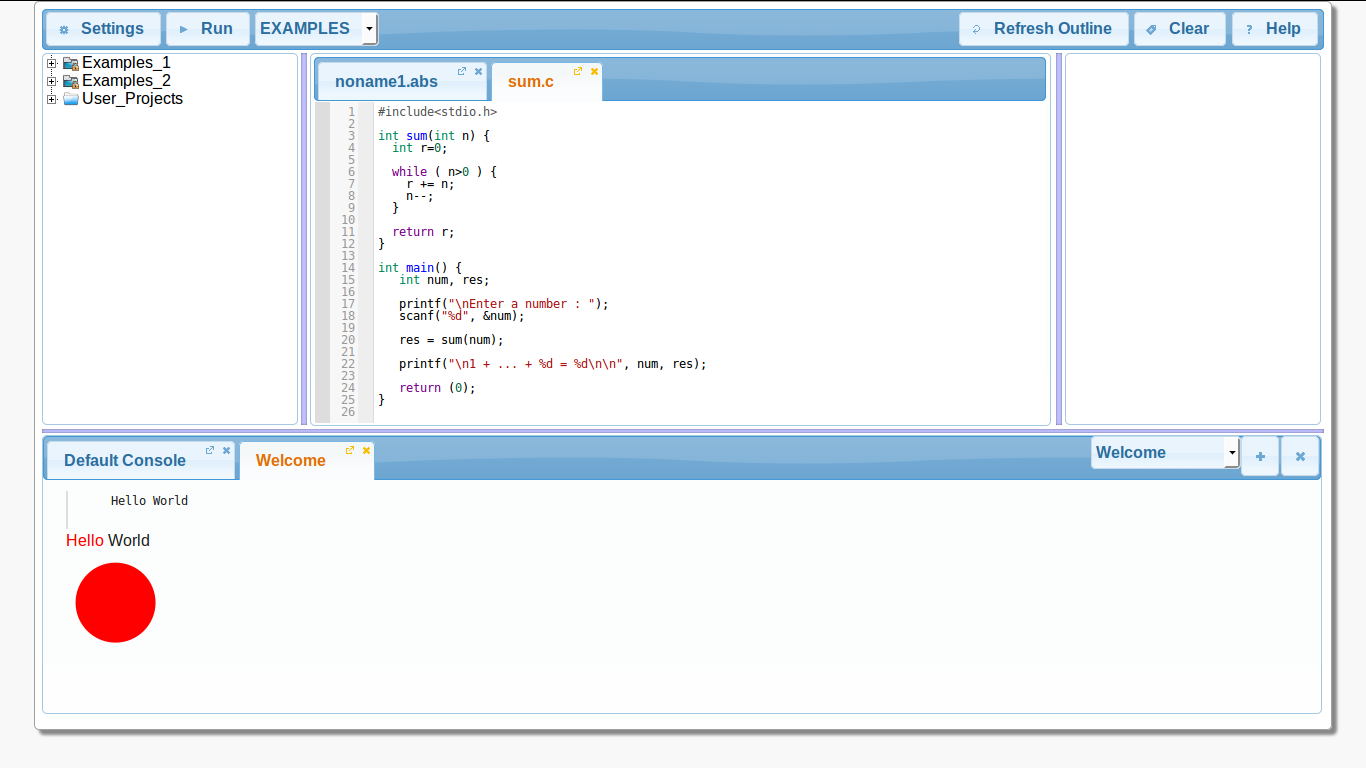
\includegraphics[width=1\textwidth]{fig/example1.png}
\end{center}
\caption{Output of Example~\ref{sec:eiol:examples:1}}
\label{fig:examples:1}
\hrule
\end{figure}
\end{example}

\begin{example}
\label{sec:eiol:examples:2}
%
The following is an example of
\xmlstructref{eiout}{oncodelineclickaction} which executes two
\xmlstructref{eiout}{highlightlinescommand}, each with different
\xmlstructattr{outclass}:

\medskip
\begin{lstlisting}
<eiactions>
 <oncodelineclick>
  <lines> <line from="3" /> </lines>
  <eicommands>
   <highlightlines outclass="info">
    <lines> <line from="2" to="4" /> </lines>
   </highlightlines>
   <highlightlines outclass="warning">
    <lines> <line from="6" fromch="4" toch="8" /> </lines>
   </highlightlines>
  </eicommands>
 </oncodelineclick>
</eiactions>
\end{lstlisting}

\medskip
\noindent
Its execution in the web-client generates the output depicted in
Figure~\ref{fig:examples:2}. Note that a click on the arrow (in the
left-side gutter) executes the commands and another click undo their
corresponding effect.


\begin{figure}[h]
\hrule\smallskip
\begin{center}
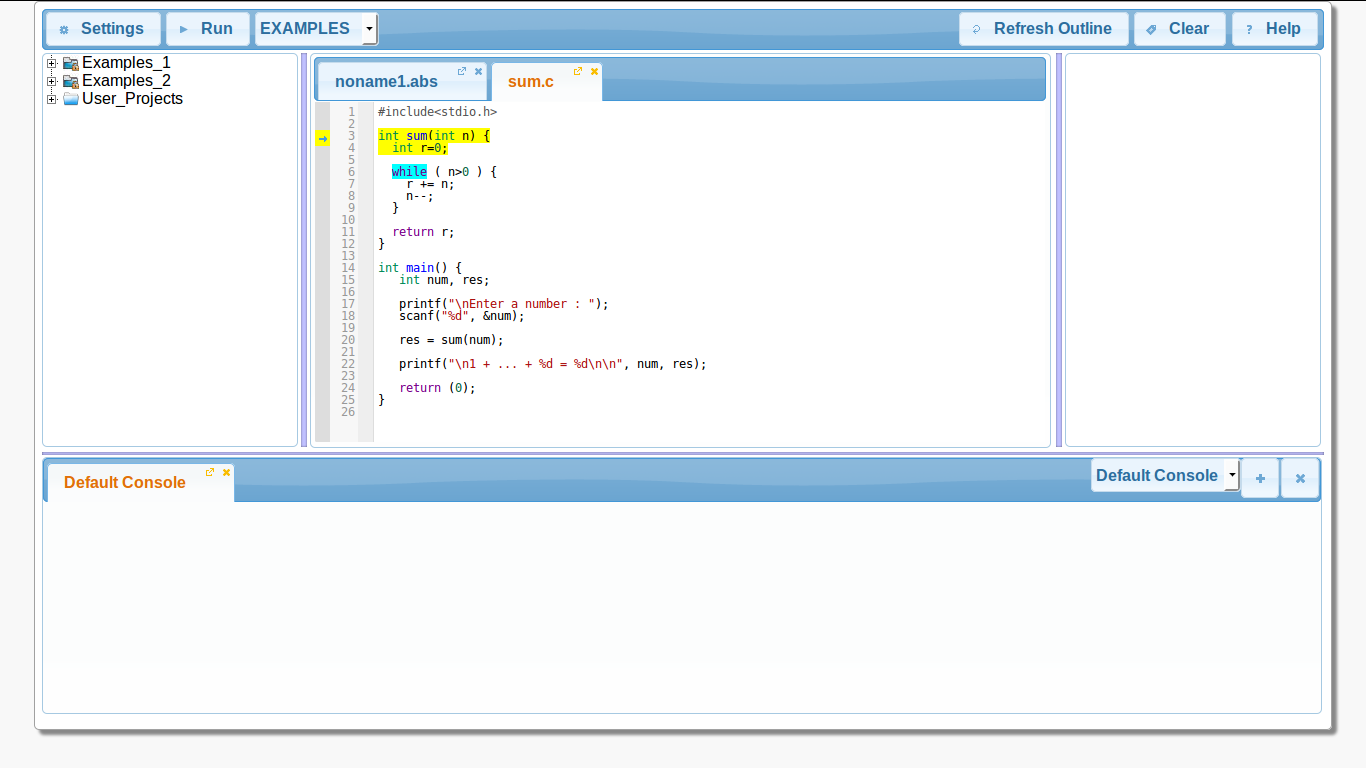
\includegraphics[width=1\textwidth]{fig/example2.png}
\end{center}
\caption{Output of Example~\ref{sec:eiol:examples:2}}
\label{fig:examples:2}
\hrule
\end{figure}
\end{example}


\begin{example}
\label{sec:eiol:examples:3}

The following is an example of \xmlstructref{eiout}{dialogboxcommand},
using a \xmlstructref{eiout}{content} environment with \lst{graph}
format.

\medskip
\begin{lstlisting}
<dialogbox boxtitle="CPU use" boxwidth="800" boxheight="500">
  <content format="graph">
    { "title":"BFS - Acer G5453",
      "f-titles":["Time","% CPU","% Mem"],
      "y-title":"%",
      "x-title":"Time",
      "groups":["BFS"],
      "labels":["Acer","G5453"],
      "values":[[1,22,43],[2,40,47],[3,82,88],[4,40,75]]
    }
    { "title":"BFS - Acer B12",
      "f-titles":["Timee","% CPU","% Mem"],
      "y-title":"%",
      "x-title":"Time",
      "groups":["BFS"],
      "labels":["Acer","B12"],
      "values":[[1,42,66],[2,65,47],[3,99,91],[4,68,92]]
    }
  </content>
</dialogbox>
\end{lstlisting}

\medskip
\noindent
Its execution in the web-client generates the output depicted in
Figure~\ref{fig:examples:3}.

\begin{figure}[h]
\hrule\smallskip
\begin{center}
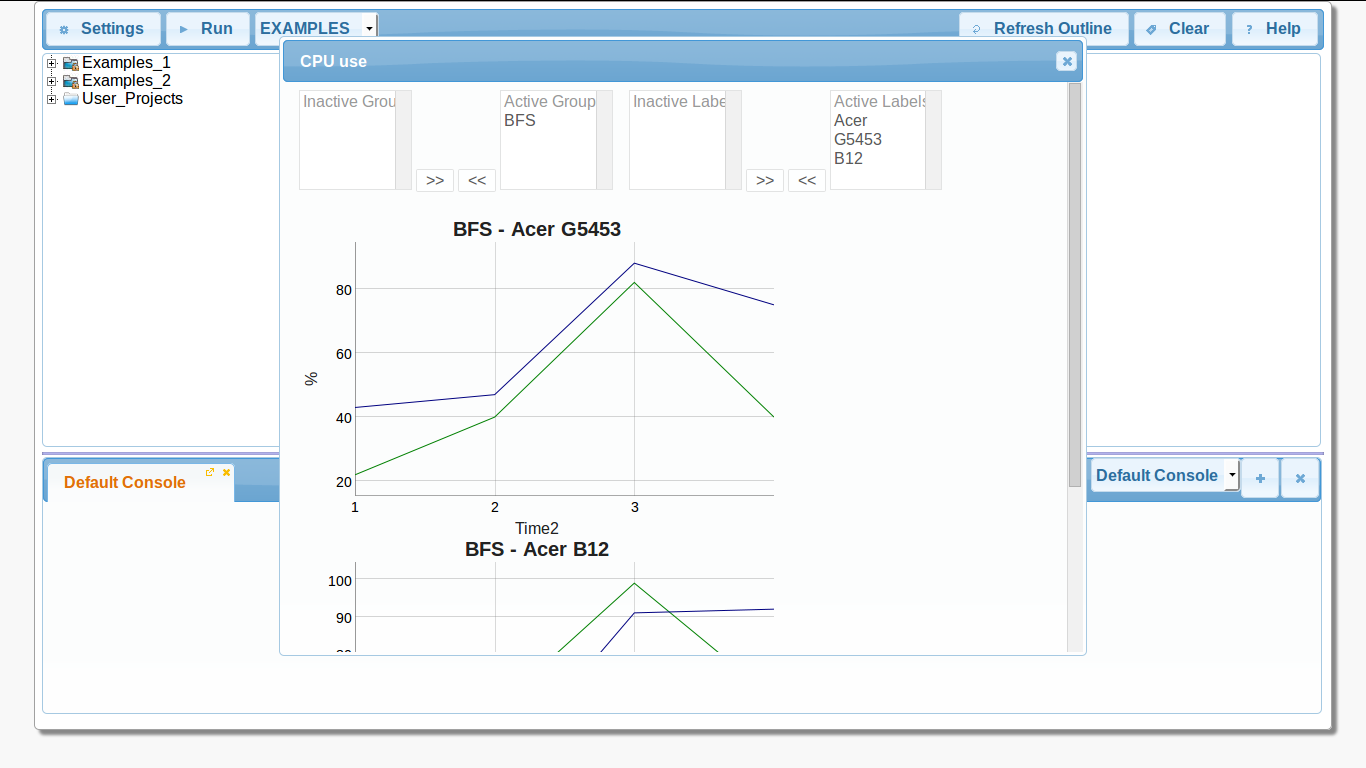
\includegraphics[width=1\textwidth]{fig/example3.png}
\end{center}
\caption{Output of Example~\ref{sec:eiol:examples:3}}
\label{fig:examples:3}
\hrule
\end{figure}

\begin{example}
\label{sec:eiol:examples:4}
%
The following is an example of \xmlstructref{eiout}{writefilecommand},
which adds a new file to the file-manager:

\medskip
\begin{lstlisting}
<writefile filename="dir1/newfile.cpp" overwrite="false">
<![CDATA[
#include <iostream>
using namespace std;
int main(){
  cout << "Hello World!" << endl;
  return 0;
}
]]>
</writefile>
\end{lstlisting}

\medskip
\noindent
Note the of \lst{<![CDATA[ ... ]]>}, this is necessary due to the use
of plain-text with special characters. Its execution in the web-client
generates the output depicted in Figure~\ref{fig:examples:4}.

\begin{figure}[h]
\hrule\smallskip
\begin{center}
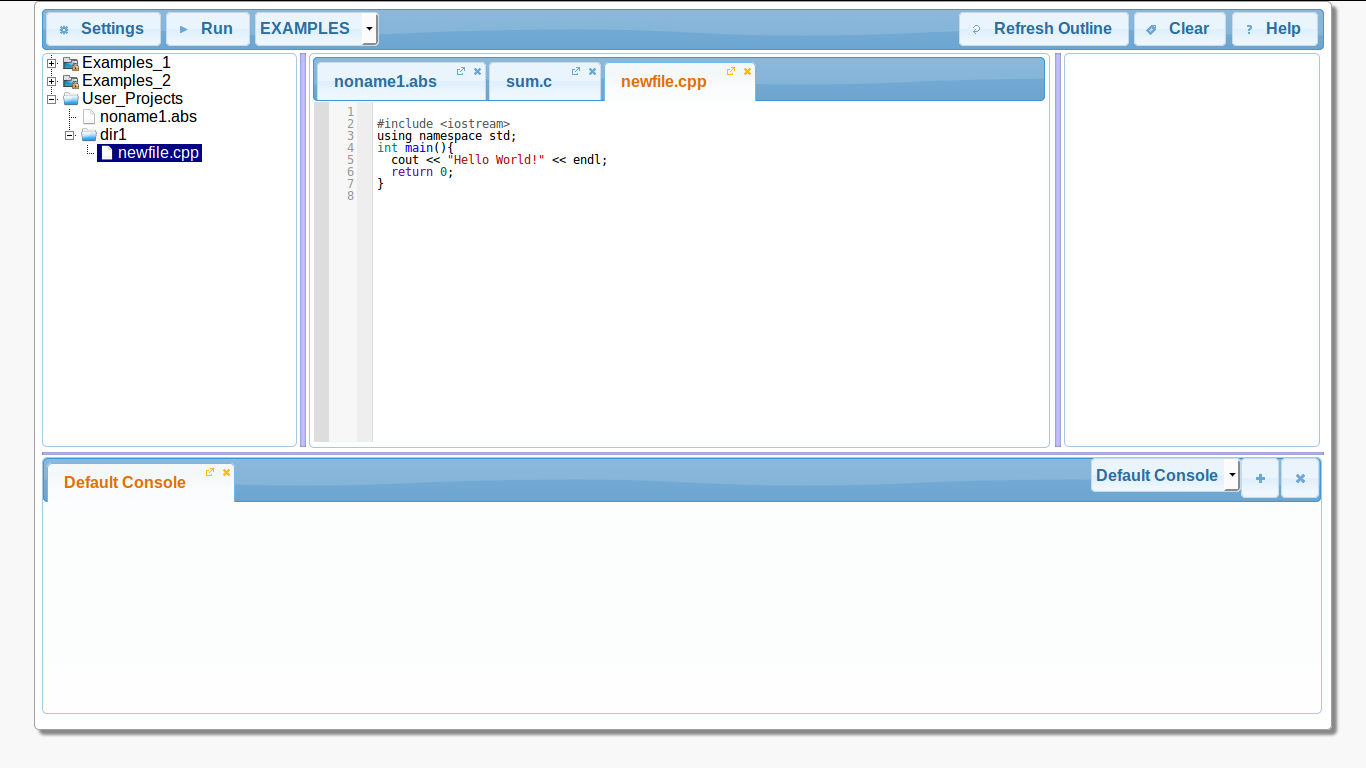
\includegraphics[width=1\textwidth]{fig/example4.png}
\end{center}
\caption{Output of Example~\ref{sec:eiol:examples:4}}
\label{fig:examples:4}
\hrule
\end{figure}
\end{example}

\end{example}

\begin{example}
\label{sec:eiol:examples:5}
%
The following is an example of \xmlstructref{eiout}{setcsscommand},
together with an action \xmlstructref{eiout}{onclickaction} which
changes the size of some text when it is clicked:

\medskip
\begin{lstlisting}
<eicommands>
 <printonconsole>
  <content format="html">
   <div id="wrap">
    <span>(*Some text*)</span><br/>
    <span id="text">Click me!</span><br/>
   </div> 
  </content>
 </printonconsole>
</eicommands>
<eiactions>
 <onclick>
  <elements>
   <selector value="#text" />
  </elements>
  <eicommands>
   <setcss>
    <elements>
     <selector value="#text" />
    </elements>
    <cssproperties>
     <cssproperty name="font-size" value="30px" />
    </cssproperties>
   </setcss>
  </eicommands>
 </onclick>
</eiactions>
\end{lstlisting}

\medskip
\noindent
Its execution in the web-client generates the output depicted in
Figure~\ref{fig:examples:5} -- it includes the result after clicking
on the text ``\lst{Click me!}''.

\begin{figure}[h]
\hrule\smallskip
\begin{center}
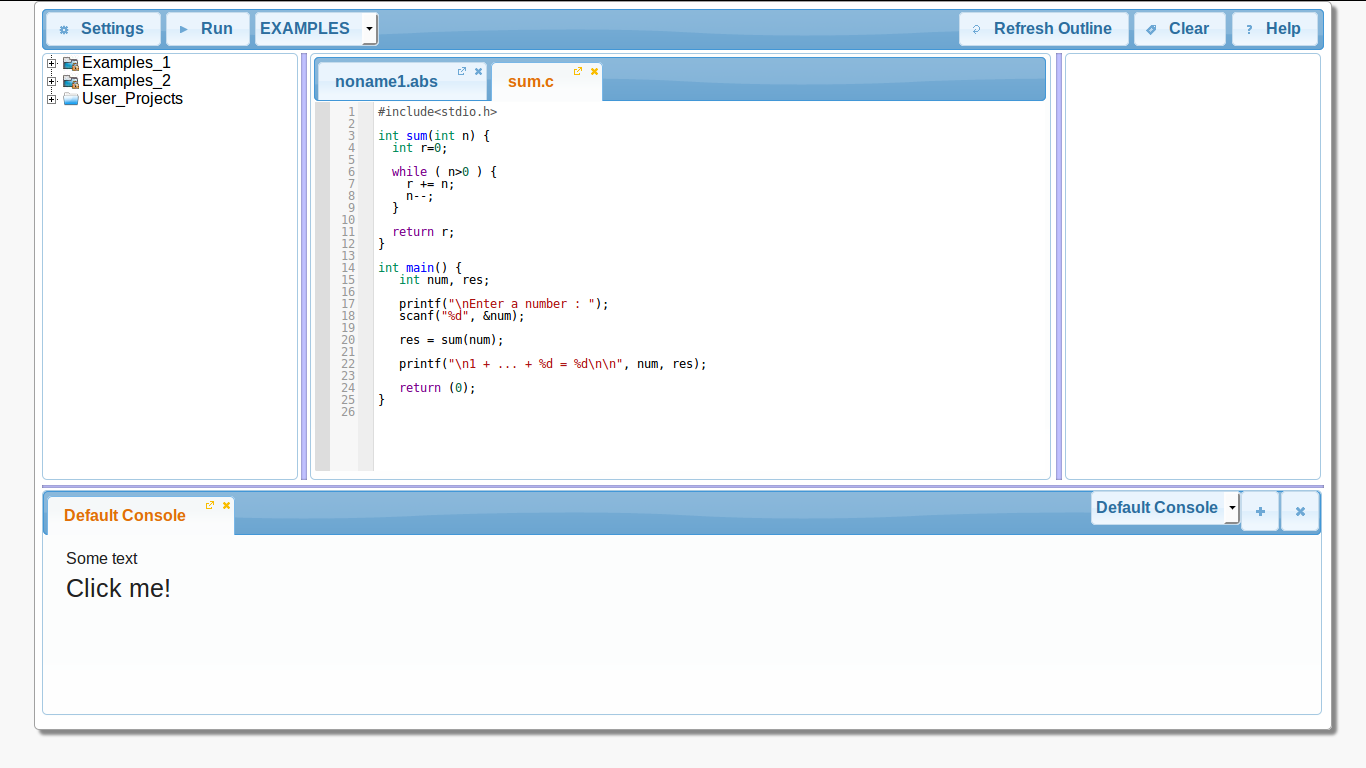
\includegraphics[width=1\textwidth]{fig/example5.png}
\end{center}
\caption{Output of Example~\ref{sec:eiol:examples:5}}
\label{fig:examples:5}
\hrule
\end{figure}
\end{example}

\begin{example}
\label{sec:eiol:examples:6}
%
The following is an example of
\xmlstructref{eiout}{changecontentcommand}. Assuming that we add the
following command to the list of commands of the
\xmlstructref{eiout}{onclickaction} in
Example~\ref{sec:eiol:examples:5}, it will add some text to the HTML
tag with identifier \lst{wrap} when ``\lst{Click me!}'' is clicked:

\medskip
\begin{lstlisting}
<changecontent action="append">
 <elements>
  <selector value="#wrap"/>
 </elements>
 <content format="html">
  <span style="color:red;">New Text added </span><br/>
 </content>
</changecontent> 
\end{lstlisting}

\medskip
\noindent
Its execution in the web-client generates the output depicted in
Figure~\ref{fig:examples:6} (after clicking on ``\lst{Click me!}'').

\begin{figure}[h]
\hrule\smallskip
\begin{center}
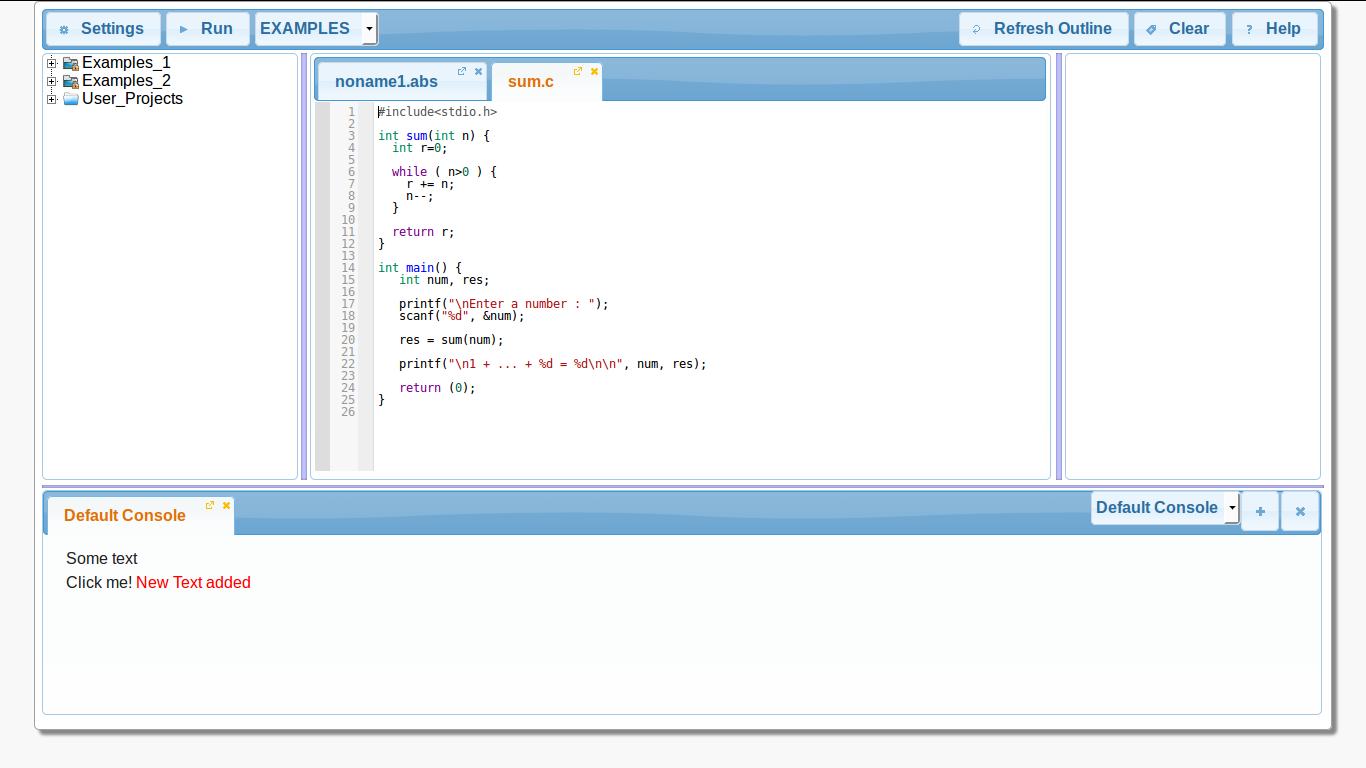
\includegraphics[width=1\textwidth]{fig/example6.png}
\end{center}
\caption{Output of Example~\ref{sec:eiol:examples:6}}
\label{fig:examples:6}
\hrule
\end{figure}
\end{example}

\begin{example}
\label{sec:eiol:examples:7}
%
The following is an example of \xmlstructref{eiout}{addmarkercommand},
using different \xmlstructattr{outclass} values:

\medskip
\begin{lstlisting}
<addmarker outclass="info">
 <lines>
  <line from="2" />
 </lines>
 <content format="text">
  Information
 </content>
</addmarker>
<addmarker outclass="warning">
 <lines>
  <line from="4" />
 </lines>
 <content format="text">
  Warning
 </content>
</addmarker>
<addmarker outclass="error">
 <lines>
  <line from="6" />
 </lines>
 <content format="text">
  Error
 </content>
</addmarker>
\end{lstlisting}

\medskip
\noindent
Its execution in the web-client generates the output depicted in
Figure~\ref{fig:examples:7}.

\begin{figure}[h]
\hrule\smallskip
\begin{center}
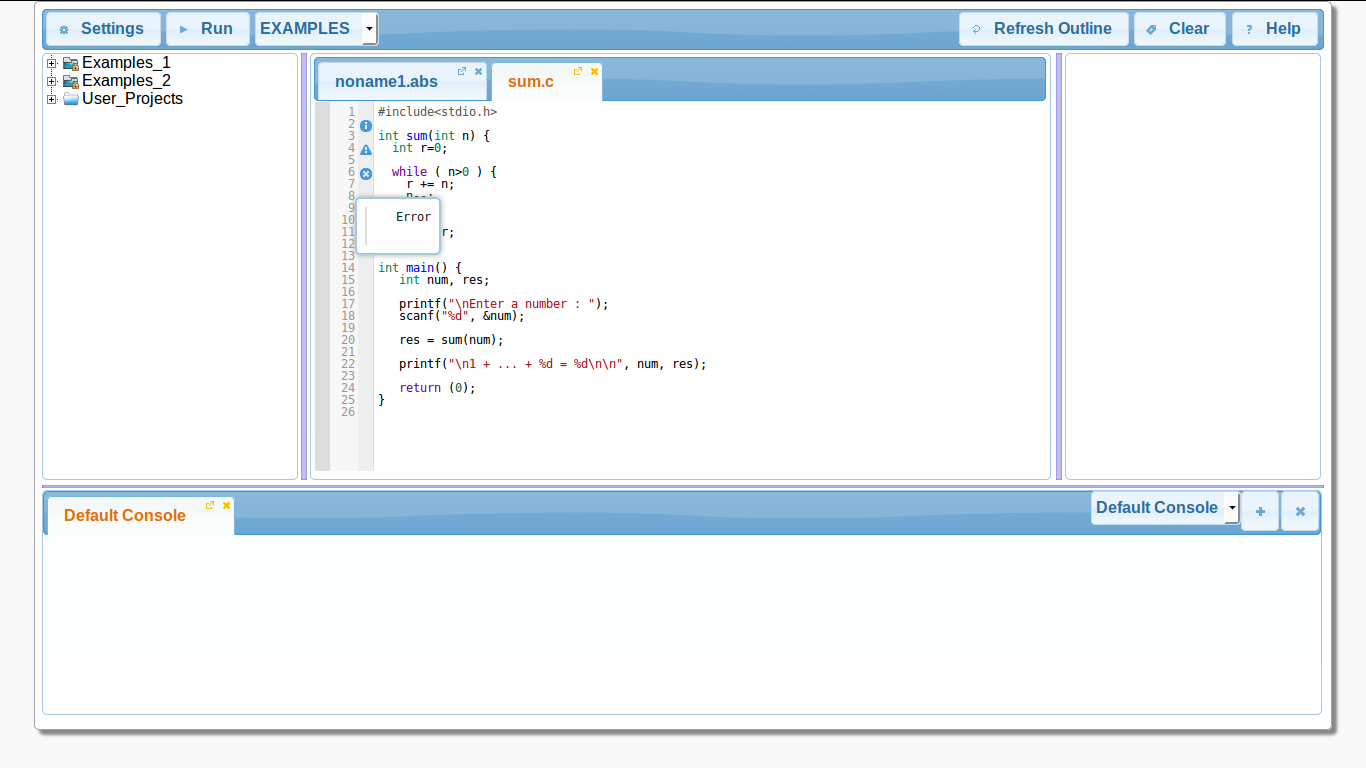
\includegraphics[width=1\textwidth]{fig/example7.png}
\end{center}
\caption{Output of Example~\ref{sec:eiol:examples:7}}
\label{fig:examples:7}
\hrule
\end{figure}
\end{example}

\begin{example}
\label{sec:eiol:examples:8}
%
The following is an example of 
\xmlstructref{eiout}{addinlinemarkercommand} using different
\xmlstructattr{outclass} values:

\medskip
\begin{lstlisting}
<addinlinemarker outclass="info">
 <lines>
  <line from="2" />
 </lines>
 <content format="text">
  Information
 </content>
</addinlinemarker>
<addinlinemarker outclass="warning">
 <lines>
  <line from="4" />
 </lines>
 <content format="text">
  Warning
 </content>
</addinlinemarker>
<addinlinemarker outclass="error">
 <lines>
  <line from="6" />
 </lines>
 <content format="text">
  Error
 </content>
</addinlinemarker>
\end{lstlisting}

\medskip
\noindent
Its execution in the web-client generates the output depicted in
Figure~\ref{fig:examples:8}.

\begin{figure}[h]
\hrule\smallskip
\begin{center}
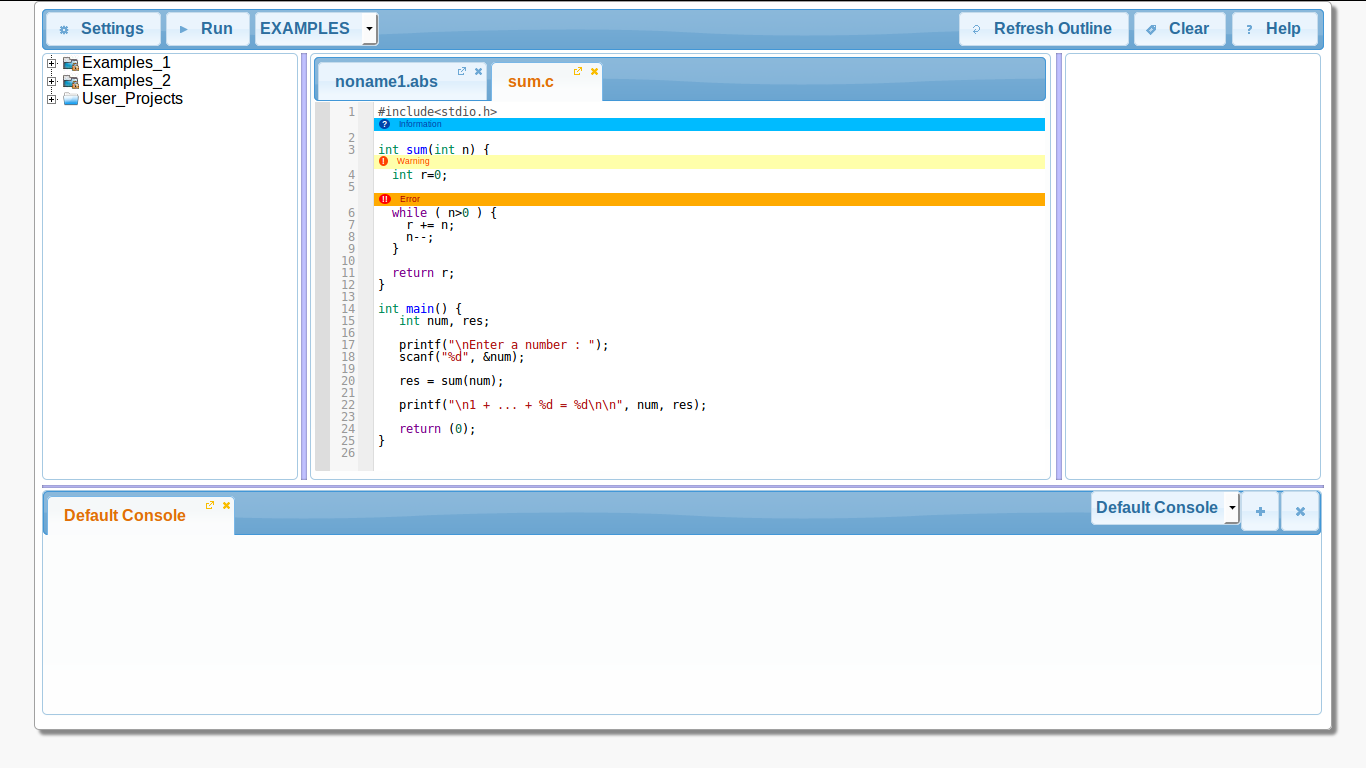
\includegraphics[width=1\textwidth]{fig/example8.png}
\end{center}
\caption{Output of Example~\ref{sec:eiol:examples:8}}
\label{fig:examples:8}
\hrule
\end{figure}
\end{example}

\begin{example}
\label{sec:eiol:examples:9}
%
The following is an example of \xmlstructref{eiout}{downloadcommand},
to download a file called \lst{$\mbox{download.test}$} generated by a
tool execution with \emph{execution identifier} \lst{xV54fga}:

\medskip
\begin{lstlisting}[mathescape=false]
<download execid="xV54fga" filename="download.test" />
\end{lstlisting}
%$
\medskip
\noindent
Its execution in the web-client generates the output as in
Figure~\ref{fig:examples:9}.

\begin{figure}[h]
\hrule\smallskip
\begin{center}
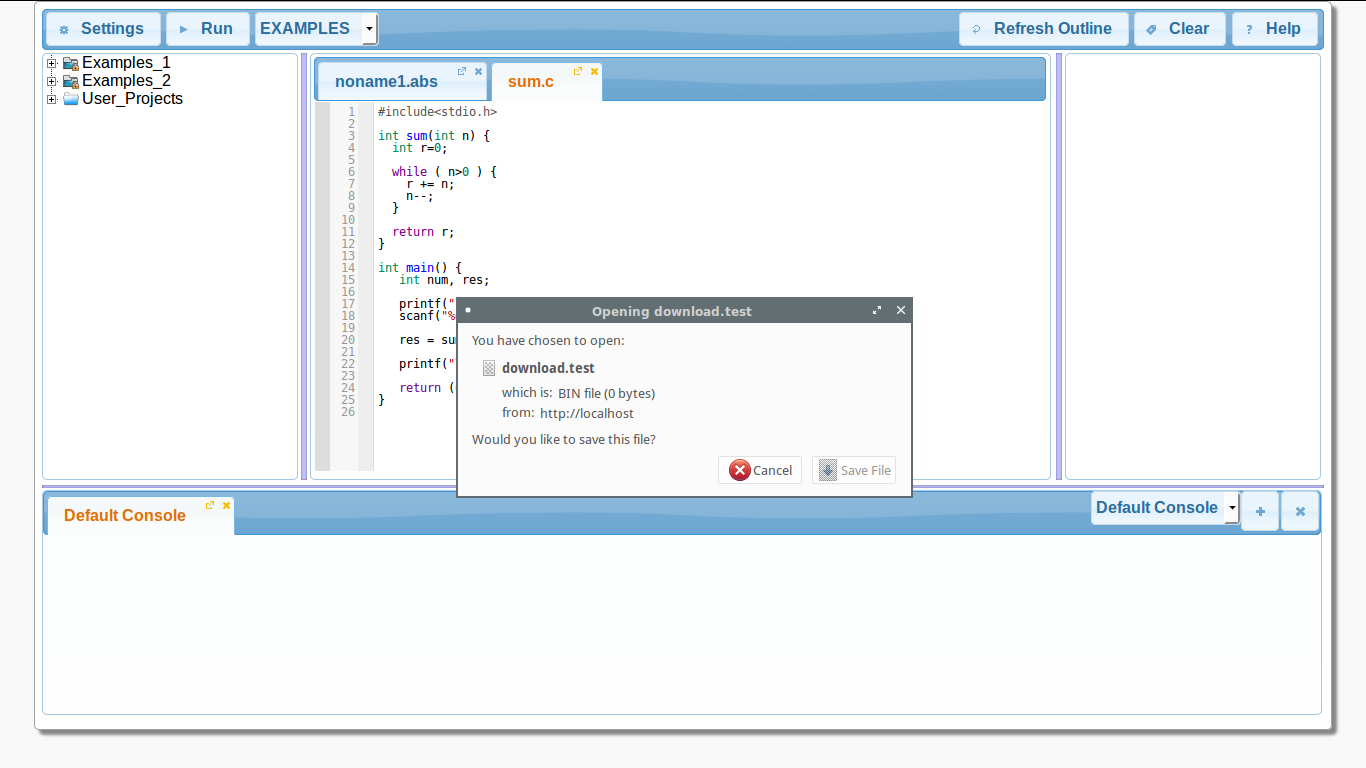
\includegraphics[width=1\textwidth]{fig/example9.png}
\end{center}
\caption{Output of Example~\ref{sec:eiol:examples:9}}
\label{fig:examples:9}
\hrule
\end{figure}
\end{example}


